% MODELO PPGMC/UESC 2.0 - Francisco Bruno Souza Oliveira (2026)
% Base: modelo 1.4, Valdex de Jesus Santos (autor) e Francisco Bruno Souza Oliveira (colaborador).
% Os creditos do template constam no README, nao no trabalho do estudante.
\documentclass[12pt,oneside,a4paper,brazil,english]{abntex2}
\usepackage[T1]{fontenc}
\usepackage[utf8]{inputenc}
\usepackage{newtxtext,newtxmath} % Times equivalente em TEXTO E MATEMATICA
\usepackage{graphicx,booktabs,amsmath,mathtools,subcaption,tabularx,array,longtable}
\usepackage[ruled,vlined,portuguese]{algorithm2e}
\usepackage{tikz}
\usetikzlibrary{arrows.meta,positioning}
\usepackage{etoolbox}
\usepackage{geometry}
\usepackage{pdfpages}
\usepackage{multicol}
\usepackage{enumitem}
\usepackage{newfloat}
\DeclareFloatingEnvironment[name=Quadro]{quadro}
\usepackage{microtype}
\usepackage{csquotes}
% Padronizacao Times-equivalente inclusive nos titulos do abntex2
\renewcommand{\ABNTEXchapterfont}{\rmfamily\bfseries}
\renewcommand{\ABNTEXchapterfontsize}{\normalsize}
\renewcommand{\ABNTEXsectionfont}{\rmfamily\bfseries}
\renewcommand{\ABNTEXsectionfontsize}{\normalsize}
\renewcommand{\ABNTEXsubsectionfont}{\rmfamily\bfseries}
\renewcommand{\ABNTEXsubsectionfontsize}{\normalsize}

\geometry{left=3cm,top=3cm,right=2cm,bottom=2cm}
\OnehalfSpacing
\setlength{\parindent}{1.25cm}
\setlength{\parskip}{0pt}
\usepackage[backend=biber,style=abnt,sorting=nyt]{biblatex}
\addbibresource{referencias.bib}
% CONFIGURACAO: altere apenas os campos a seguir.
% mestrado/doutorado; qualificacao/defesa
\def\Modalidade{mestrado}
\def\Etapa{qualificacao}
\def\Autor{Nome Completo do Estudante}
\def\Titulo{Modelagem computacional de um problema de transporte}
\def\Cidade{Ilhéus -- BA}
\def\Ano{2026}
\def\DataBanca{22 de outubro de 2026}
\def\Orientador{Prof. Dr. Nome do Orientador}
\def\InstOrientador{UESC}
\def\Coorientador{}
\def\InstCoorientador{UESC}
\def\ExaminadorA{Prof. Dr. Examinador A}
\def\InstA{UESC / PPGMC}
\def\ExaminadorB{Prof. Dr. Examinador B}
\def\InstB{Instituição externa ao PPGMC e, na defesa, externa à UESC}
\def\ExaminadorC{Prof. Dr. Examinador C}
\def\InstC{UESC}
\def\ExaminadorD{Prof. Dr. Examinador D}
\def\InstD{Instituição externa à UESC}
\def\AreaConcentracao{Área de concentração conforme cadastro oficial}
\def\LinhaPesquisa{Linha de pesquisa conforme cadastro oficial}
% Para a ficha catalografica: coloque o PDF na pasta pretextuais,
% com o nome ficha-catalografica.pdf e descomente a linha de inclusao em main.tex na versao final.

\hypersetup{hidelinks,pdfauthor={\Autor},pdftitle={\Titulo}}
\newbool{doutorado}\newbool{qualificacao}
\ifdefstring{\Modalidade}{doutorado}{\booltrue{doutorado}}{\boolfalse{doutorado}}
\ifdefstring{\Etapa}{qualificacao}{\booltrue{qualificacao}}{\boolfalse{qualificacao}}
\newcommand{\Tipotrabalho}{\ifbool{doutorado}{Tese}{Dissertação}}
\newcommand{\Tipopreliminar}{\ifbool{doutorado}{tese}{dissertação}}
\titulo{\Titulo}\autor{\Autor}\local{\Cidade}\data{\Ano}
\instituicao{Universidade Estadual de Santa Cruz\\Programa de Pós-Graduação em Modelagem Computacional em Ciência e Tecnologia}
\tipotrabalho{\Tipotrabalho}
\preambulo{\ifbool{qualificacao}{Versão preliminar da \Tipopreliminar\ apresentada ao Programa de Pós-Graduação em Modelagem Computacional em Ciência e Tecnologia da Universidade Estadual de Santa Cruz para exame de qualificação.}{\Tipotrabalho\ apresentada ao Programa de Pós-Graduação em Modelagem Computacional em Ciência e Tecnologia da Universidade Estadual de Santa Cruz como parte dos requisitos para obtenção do título correspondente.}\\Área de concentração: \AreaConcentracao.}
\newcommand{\Membro}[3]{\par\vspace{0.44cm}\noindent\rule{10cm}{0.4pt}\\#1\\{\small #2 --- #3}\par}
\newcommand{\FolhaBanca}{%
\cleardoublepage\thispagestyle{empty}\begin{center}\textbf{\Autor}\\[0.7cm]\textbf{\Titulo}\\[0.6cm]
\ifbool{qualificacao}{\textbf{BANCA DO EXAME DE QUALIFICAÇÃO}}{\textbf{FOLHA DE APROVAÇÃO}}\end{center}
\noindent\ifbool{qualificacao}{Exame de qualificação da versão preliminar da \Tipopreliminar.}{\Tipotrabalho\ apresentada ao PPGMC/UESC para obtenção do título correspondente.}\\[0.2cm]Data: \DataBanca.\par
\Membro{\Orientador}{Presidente / Orientador}{\InstOrientador}
\ifdefempty{\Coorientador}{}{\Membro{\Coorientador}{Coorientador (participação adicional; consultar homologação)}{\InstCoorientador}}
\Membro{\ExaminadorA}{\ifbool{qualificacao}{Membro interno ao PPGMC}{Membro interno à UESC}}{\InstA}
\Membro{\ExaminadorB}{\ifbool{qualificacao}{Membro externo ao PPGMC}{Membro externo à UESC}}{\InstB}
\ifbool{qualificacao}{}{\ifbool{doutorado}{\Membro{\ExaminadorC}{Membro interno à UESC}{\InstC}\Membro{\ExaminadorD}{Membro externo à UESC}{\InstD}}{}}
\clearpage}
\begin{document}
\pretextual
\begin{capa}\begin{center}

\includegraphics[width=6cm]{figuras/logo-ppgmc-original-adaptado.png}\\[0.15cm]

\includegraphics[height=1.7cm]{figuras/brasao-uesc-oficial.png}\\[0.35cm]
{\bfseries UNIVERSIDADE ESTADUAL DE SANTA CRUZ}\\
{\bfseries PROGRAMA DE PÓS-GRADUAÇÃO EM MODELAGEM COMPUTACIONAL EM CIÊNCIA E TECNOLOGIA}
\vfill{\bfseries\Autor}\vfill{\bfseries\Titulo}\\[0.5cm]
\ifbool{qualificacao}{\textbf{VERSÃO PRELIMINAR PARA QUALIFICAÇÃO}}{}\vfill\Cidade\\\Ano
\end{center}\end{capa}
\imprimirfolhaderosto*
% Para inserir a ficha oficial, descomente a linha abaixo apos adicionar o PDF:
% \includepdf[pages=1]{pretextuais/ficha-catalografica.pdf}
\FolhaBanca
\begin{dedicatoria}\vspace*{\fill}\begin{flushright}Espaço reservado à dedicatória (opcional).\end{flushright}\end{dedicatoria}

\begin{agradecimentos}Agradeço às pessoas e instituições que contribuíram para o desenvolvimento desta pesquisa. Este texto é demonstrativo e deve ser substituído pelo estudante.\end{agradecimentos}

\begin{epigrafe}\vspace*{\fill}\begin{flushright}\textit{Espaço reservado à epígrafe, se desejada.}\end{flushright}\end{epigrafe}

\begin{resumo}Este documento demonstra a organizacao do modelo PPGMC 2.0. O conteudo e ilustrativo e deve ser substituido pela descricao da pesquisa efetivamente realizada.\\
\textbf{Palavras-chave}: modelagem computacional; interdisciplinaridade; metodos numericos.
\end{resumo}
\begin{resumo}[Abstract]\begin{otherlanguage*}{english}This document illustrates the PPGMC 2.0 template. All sample content must be replaced with the student's actual research.\\
\textbf{Keywords}: computational modeling; interdisciplinarity; numerical methods.
\end{otherlanguage*}\end{resumo}
\listoffigures*\cleardoublepage
\listoftables*\cleardoublepage
\begin{siglas}\item[UESC] Universidade Estadual de Santa Cruz\item[PPGMC] Programa de Pós-Graduação em Modelagem Computacional em Ciência e Tecnologia\item[HPC] Computação de Alto Desempenho\end{siglas}
\begin{simbolos}\item[$\Omega$] Domínio computacional\item[$h$] Tamanho característico da malha\item[$\phi$] Campo escalar de interesse\end{simbolos}


\tableofcontents*\cleardoublepage
\textual
\chapter{Introdução}\label{chap:introducao}
Este documento apresenta um exemplo de dissertação, tese ou relatório de qualificação do PPGMC/UESC. A versão 2.0 preserva a vocação didática da versão 1.4: além de servir como ponto de partida, demonstra os principais recursos de escrita científica em \LaTeX. O conteúdo exemplificativo deve ser substituído pelo trabalho do estudante.

A modelagem computacional permite investigar fenômenos por meio de modelos matemáticos, discretizações e algoritmos. Um problema científico envolve perguntas de pesquisa, hipóteses, dados, métodos e critérios de validação. A introdução deve delimitar o problema, explicitar sua relevância e apresentar o percurso argumentativo.

\section{Contextualização e motivação}
A descrição do problema deve indicar o contexto científico, o estado do conhecimento e a lacuna investigada. Recomenda-se fundamentar afirmações relevantes com fontes bibliográficas verificáveis. A construção de modelos deve explicitar hipóteses, escalas e limites de aplicabilidade.

\section{Problema de pesquisa e justificativa}
O estudante deve formular uma pergunta clara, justificar sua relevância e identificar as contribuições esperadas. Evite confundir a utilização de uma ferramenta com o objetivo científico da investigação.

\section{Objetivos}
\subsection{Objetivo geral}
Investigar, por meio de modelagem computacional, um fenômeno de interesse, explicitando hipóteses e critérios de avaliação.
\subsection{Objetivos específicos}
\begin{enumerate}[label=\alph*)]
\item Formular um modelo matemático apropriado ao problema.
\item Implementar e verificar uma solução computacional.
\item Avaliar os resultados e as limitações do método.
\end{enumerate}

\section{Interdisciplinaridade da pesquisa}
A interdisciplinaridade deve ser apresentada como integração efetiva de contribuições, e não apenas como uma lista de áreas. No exemplo da Figura~\ref{fig:interdisciplinaridade}, a Física descreve fenômenos, a Matemática fornece modelos e métodos, a Computação viabiliza algoritmos e a Engenharia Nuclear estabelece aplicações e requisitos de validação. O estudante deve substituir as áreas e as contribuições pelas que realmente integram seu trabalho.
\begin{figure}[htbp]\centering
\resizebox{\textwidth}{!}{% Edite os quatro pares: nome da área / contribuição.
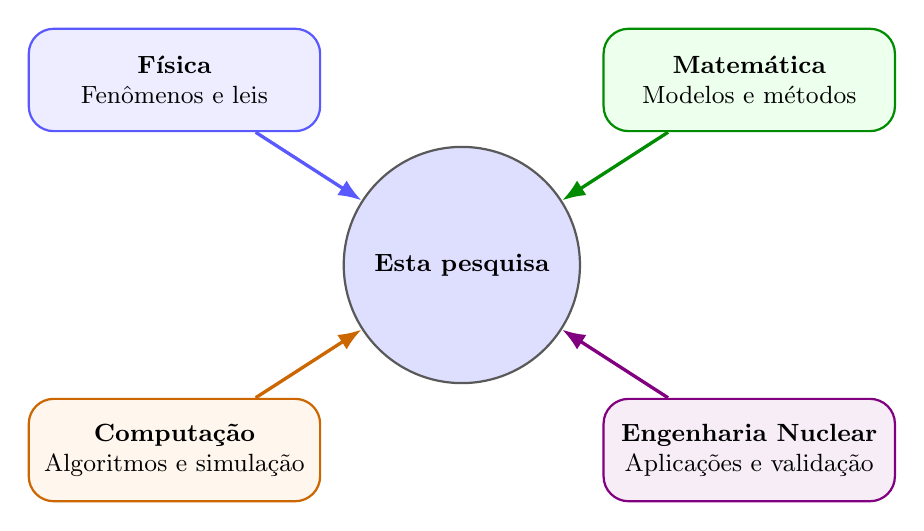
\begin{tikzpicture}[>=Latex, every node/.style={align=center,font=\small},
 area/.style={draw,rounded corners=9pt,minimum width=3.7cm,minimum height=1.3cm,thick},
 central/.style={circle,draw=black!65,fill=blue!13,minimum size=3cm,thick}]
\node[central] (p) at (0,0) {\textbf{Esta pesquisa}};
\node[area,draw=blue!65,fill=blue!7] (a) at (-3.65,2.35) {\textbf{Física}\\Fenômenos e leis};
\node[area,draw=green!55!black,fill=green!7] (b) at (3.65,2.35) {\textbf{Matemática}\\Modelos e métodos};
\node[area,draw=orange!80!black,fill=orange!7] (c) at (-3.65,-2.35) {\textbf{Computação}\\Algoritmos e simulação};
\node[area,draw=violet,fill=violet!7] (d) at (3.65,-2.35) {\textbf{Engenharia Nuclear}\\Aplicações e validação};
\draw[->,very thick,blue!65] (a) -- (p);
\draw[->,very thick,green!55!black] (b) -- (p);
\draw[->,very thick,orange!80!black] (c) -- (p);
\draw[->,very thick,violet] (d) -- (p);
\end{tikzpicture}
}
\caption{Exemplo editável de integração interdisciplinar em uma pesquisa.}\label{fig:interdisciplinaridade}
\fonte{Elaboração própria (exemplo didático).}
\end{figure}

\section{Organização do documento}
O Capítulo~\ref{chap:organizacao} explica os arquivos do projeto; o Capítulo~\ref{chap:citacoes} apresenta citações e referências; o Capítulo~\ref{chap:elementos} reúne figuras, quadros, tabelas, equações e algoritmos; os capítulos seguintes exemplificam metodologia, resultados e conclusão. No modo qualificação, acrescenta-se um cronograma de atividades.

\chapter{Organização dos arquivos e configuração}\label{chap:organizacao}
O arquivo principal é \texttt{main.tex}. A classe de documento é \texttt{abntex2}, com personalizações para o PPGMC. A configuração centralizada está no arquivo \texttt{configuracao.tex}. Os capítulos são arquivos independentes na pasta \texttt{capitulos}, permitindo escrita progressiva e colaboração.

\section{Escolha da modalidade}
No arquivo de configuração, use \verb|\def\Modalidade{mestrado}| ou \verb|\def\Modalidade{doutorado}|. Para escolher a etapa, use \verb|\def\Etapa{qualificacao}| ou \verb|\def\Etapa{defesa}|. O modelo produz automaticamente a apresentação correspondente.

\section{Elementos pré-textuais}
A capa, a folha de rosto e a folha de banca são produzidas pelo arquivo principal. Dedicatória, agradecimentos e epígrafe são exemplos opcionais, editáveis na pasta \texttt{pretextuais}. O resumo e o \textit{abstract} devem sintetizar o trabalho efetivamente realizado. As listas e o sumário são gerados automaticamente.

\subsection{Ficha catalográfica}
Na versão definitiva, insira o arquivo oficial fornecido pelo setor competente no caminho \texttt{pretextuais/ficha-catalografica.pdf}. A configuração \verb|\def\IncluirFicha{true}| ativa sua inclusão. Não gere dados catalográficos fictícios.

\section{Folhas de banca}
Para defesa de mestrado, o padrão contém três examinadores, incluindo o orientador e pelo menos um externo à UESC. Para defesa de doutorado, cinco examinadores, incluindo o orientador e pelo menos dois externos à UESC. A qualificação requer ao menos três especialistas, incluindo o orientador e um externo ao PPGMC; coorientadores não contam para esse mínimo. A composição efetiva deve ser homologada pelo Colegiado. A folha de qualificação não substitui a ata de avaliação.

\section{Arquivos textuais e pós-textuais}
Cada capítulo tem seu arquivo próprio. As referências são armazenadas em \texttt{referencias.bib}; apêndices e anexos ficam em pastas separadas. Evite alterar comandos estruturais no arquivo principal, salvo quando necessário.

\section{Compilação no Overleaf}
Configure o compilador \textbf{pdfLaTeX} e o processador bibliográfico \textbf{Biber}. Na linha de comando, execute \texttt{pdflatex main}, \texttt{biber main} e duas vezes \texttt{pdflatex main}. A última passagem resolve referências cruzadas, numeração e sumário.

\chapter{Citações e referências}\label{chap:citacoes}
Citações permitem reconhecer fontes, delimitar o conhecimento existente e fundamentar argumentos. Este exemplo utiliza o sistema autor-data e um arquivo bibliográfico externo. A apresentação deve ser verificada conforme as edições vigentes da ABNT, particularmente a NBR 10520:2023 e a NBR 6023:2025.

\section{Referências no arquivo bibliográfico}
O arquivo \texttt{referencias.bib} reúne os metadados. Use os tipos \texttt{@book}, \texttt{@article}, \texttt{@inproceedings} e \texttt{@online}, conforme o material citado. Para artigos científicos, registre título, periódico, ano, volume, número, páginas e DOI quando disponíveis.

\section{Citações indiretas}
Uma citação narrativa pode ser construída com \verb|\textcite{knuth1984a}|, como em \textcite{knuth1984a}, que discute programação literária. Para citações entre parênteses, use \verb|\parencite{lamport1994}|, produzindo \parencite{lamport1994}. A indicação de fontes múltiplas deve ser coerente com a norma adotada \parencite{knuth1984a,lamport1994}.

\section{Citações diretas curtas}
Uma citação direta curta integra o parágrafo, entre aspas, acompanhada da indicação da fonte e da localização correspondente. \textbf{Não invente citações textuais nem números de página.} Para demonstrar o comando sem atribuir uma frase inexistente a um autor, considere a sintaxe \verb|\parencite[p.~12]{chave}| e substitua a chave e a página por dados efetivamente conferidos.

\section{Citações diretas longas}
As citações longas são destacadas em bloco, com recuo e espaçamento apropriados. O exemplo abaixo contém texto instrutivo próprio, não uma transcrição bibliográfica:
\begin{citacao}
Este espaço demonstra a formatação de uma citação longa. Ao utilizar o ambiente em uma dissertação ou tese, substitua este texto por transcrição fiel de uma fonte consultada, identificando autor, ano e página conforme a norma vigente.
\end{citacao}

\section{Fontes digitais, DOI e conferência}
Antes de entregar o documento, confirme a correspondência entre citações e referências, a integridade de endereços eletrônicos, a forma de apresentação dos identificadores digitais e os dados de autoria. O estilo automatizado reduz o trabalho, mas não substitui a conferência normativa.

\section{Exemplo de entrada bibliográfica}
\begin{verbatim}
@book{lamport1994,
  author    = {Leslie Lamport},
  title     = {LaTeX: A Document Preparation System},
  edition   = {2},
  publisher = {Addison-Wesley},
  year      = {1994}
}
\end{verbatim}

\chapter{Figuras, tabelas, quadros, equações e algoritmos}\label{chap:elementos}
Este capítulo retoma os exemplos práticos da versão 1.4. Figuras, tabelas, equações e algoritmos recebem numeração automática e podem ser citados com \verb|\label| e \verb|\ref|. O conteúdo foi reorganizado para facilitar a substituição pelos elementos da pesquisa.

\section{Figuras}
A Figura~\ref{fig:uesc} apresenta o brasão institucional utilizado como exemplo. A identificação da fonte deve acompanhar a figura.
\begin{figure}[htbp]\centering

\includegraphics[width=0.27\textwidth]{figuras/brasao-uesc-oficial.png}
\caption{Brasão da Universidade Estadual de Santa Cruz.}\label{fig:uesc}
\fonte{Material institucional do modelo original.}
\end{figure}

\subsection{Figuras lado a lado}
A Figura~\ref{fig:comparacao} ilustra o uso de subfiguras, preservando as imagens exemplificativas do projeto 1.4. As legendas históricas originais são mantidas apenas como demonstração de composição visual, sem afirmação de data ou proveniência das fotografias.
\begin{figure}[htbp]\centering
\begin{subfigure}[b]{0.43\textwidth}\centering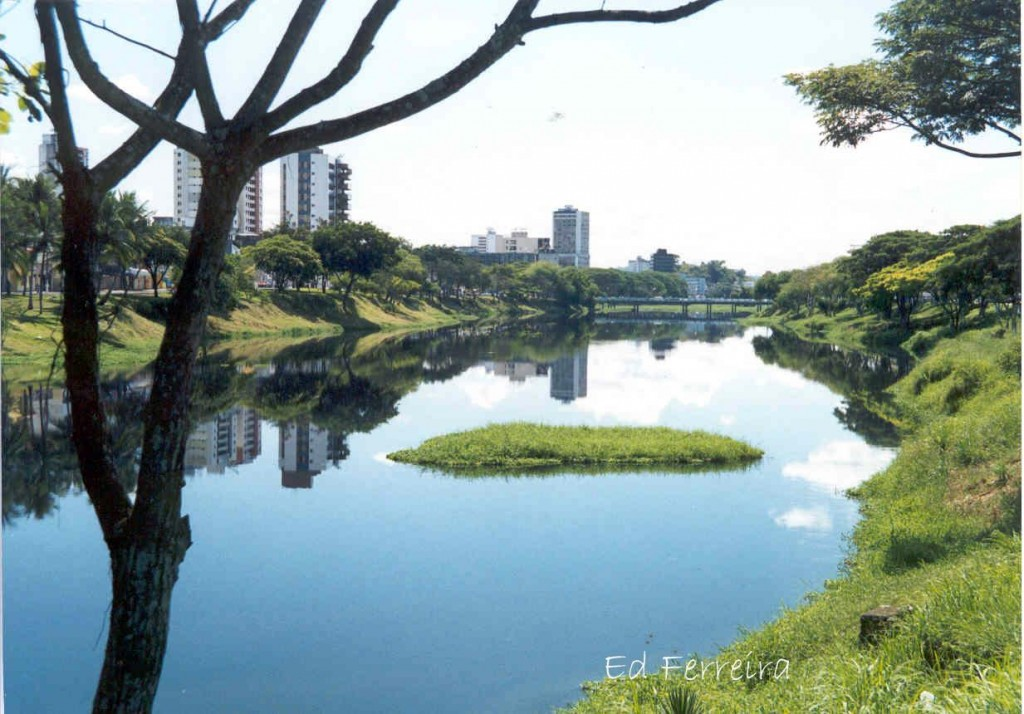
\includegraphics[width=\linewidth]{figuras/rc-adezanos.jpg}\caption{Imagem A.}\end{subfigure}\hfill
\begin{subfigure}[b]{0.43\textwidth}\centering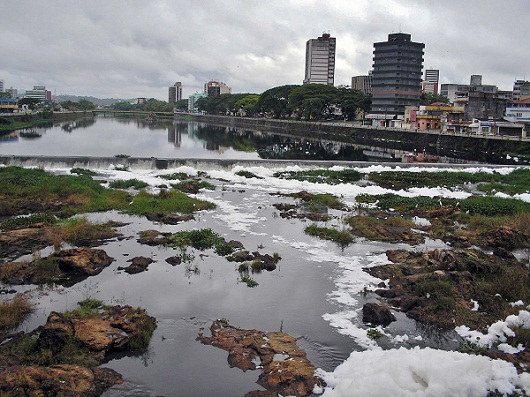
\includegraphics[width=\linewidth]{figuras/rc-atualmente.jpg}\caption{Imagem B.}\end{subfigure}
\caption{Exemplo de comparação de imagens lado a lado.}\label{fig:comparacao}
\fonte{Imagens demonstrativas preservadas da versão 1.4; proveniência a conferir.}
\end{figure}

\section{Quadros e tabelas}
O Quadro~\ref{qua:comparacao} organiza informações qualitativas, enquanto a Tabela~\ref{tab:resultados} apresenta dados numéricos ilustrativos. Não trate os valores de exemplo como resultados científicos.
\begin{quadro}[htbp]\centering\caption{Comparação qualitativa de abordagens.}\label{qua:comparacao}
\begin{tabularx}{\textwidth}{|X|X|}\hline
\textbf{Abordagem A} & \textbf{Abordagem B}\\\hline
Implementação de referência. & Implementação alternativa.\\\hline
Ênfase na precisão. & Ênfase no custo computacional.\\\hline
\end{tabularx}\\[2pt]\fonte{Elaboração própria; exemplo didático.}
\end{quadro}

\begin{table}[htbp]\centering\caption{Resultados numéricos demonstrativos.}\label{tab:resultados}
\begin{tabular}{lrrr}\toprule Caso & Erro & Tempo (s) & Iterações\\\midrule
A & 0,012 & 1,80 & 120\\
B & 0,008 & 2,40 & 180\\
C & 0,005 & 3,10 & 240\\\bottomrule
\end{tabular}\\[2pt]\fonte{Valores fictícios exclusivamente para exemplificar a formatação.}
\end{table}

\section{Equações e sistemas}
A transformada de Laplace da função $x(t)$ é apresentada na Equação~\ref{eq:laplace}:
\begin{equation}\label{eq:laplace}X(s)=\int_0^\infty x(t)e^{-st}\,\mathrm{d}t.\end{equation}
A transformada discreta de Fourier bidimensional pode ser escrita como
\begin{equation}\label{eq:dft}F(u,v)=\sum_{m=0}^{M-1}\sum_{n=0}^{N-1}f(m,n)\exp\!\left[-2\pi i\left(\frac{um}{M}+\frac{vn}{N}\right)\right].\end{equation}
Um sistema linear e uma matriz de exemplo são representados por
\begin{equation}\label{eq:sistema}A\mathbf{x}=\mathbf{b},\qquad A=\begin{bmatrix}2&-1\\-1&2\end{bmatrix},\quad \mathbf{b}=\begin{bmatrix}1\\0\end{bmatrix}.\end{equation}

\section{Algoritmos}
O Algoritmo~\ref{alg:iterativo} exemplifica a escrita de pseudocódigo com entrada, saída, condição e laço. A lógica é ilustrativa e não substitui um método de pesquisa validado.
\begin{algorithm}[htbp]
\caption{Iteração com critério de parada}\label{alg:iterativo}
\KwIn{Aproximação inicial $x_0$, tolerância $\varepsilon$, limite $N$}
\KwOut{Aproximação $x$}
$x\leftarrow x_0$; $k\leftarrow 0$\;
\While{$k<N$}{
 calcular $x_{\mathrm{novo}}$ a partir de $x$\;
 \If{$\lVert x_{\mathrm{novo}}-x\rVert<\varepsilon$}{\Return $x_{\mathrm{novo}}$\;}
 $x\leftarrow x_{\mathrm{novo}}$\; $k\leftarrow k+1$\;
}
\Return $x$\;
\end{algorithm}

\subsection{Comandos úteis para algoritmos}
O pacote \texttt{algorithm2e} oferece estruturas como \verb|\While|, \verb|\For|, \verb|\If| e \verb|\KwIn|. Os ambientes devem ser acompanhados de legenda e referência cruzada quando citados no texto.

\chapter{Metodologia}\label{chap:metodologia}
A metodologia deve permitir compreender e reproduzir o percurso científico. Recomenda-se explicitar hipóteses, formulação matemática, condições de contorno, discretização, algoritmos, parâmetros, infraestrutura e métricas de avaliação.

\section{Formulação do problema}
Considere um domínio $\Omega$ e uma variável de estado $\phi$. Um modelo genérico pode ser representado por
\begin{equation}\label{eq:modelo}\mathcal{L}(\phi;\boldsymbol{\theta})=f\quad\text{em }\Omega,\end{equation}
em que $\mathcal{L}$ é um operador, $\boldsymbol{\theta}$ representa parâmetros e $f$ é um termo de fonte. Esta equação é um exemplo abstrato, não uma descrição de um experimento realizado.

\section{Discretização e implementação}
O estudante deve identificar malha, passo temporal, tolerâncias, bibliotecas utilizadas e versões dos programas. Para modelos computacionais, registre critérios de convergência e a forma de verificação do código.

\section{Verificação e validação}
Verificação e validação respondem a perguntas distintas: se as equações discretizadas foram resolvidas corretamente e se o modelo representa adequadamente o fenômeno de interesse. Descreva testes, soluções de referência, incertezas e limitações.

\section{Reprodutibilidade}
Informe a origem dos dados, os procedimentos de processamento e a disponibilidade de código, quando pertinente. Use tabelas para reunir parâmetros e apresente claramente o ambiente computacional.

\chapter{Resultados e discussão}\label{chap:resultados}
Este capítulo é um roteiro de apresentação dos resultados. Em trabalhos reais, as figuras e tabelas devem refletir dados efetivamente obtidos e conter discussão compatível com os objetivos definidos.

\section{Organização dos experimentos}
Defina cenários, parâmetros de controle e critérios de comparação. Indique quais resultados são quantitativos, qualitativos ou exploratórios.

\section{Apresentação e análise}
A Tabela~\ref{tab:resultados} demonstra como organizar métricas, mas seus valores são fictícios. Em uma pesquisa real, substitua-a por dados rastreáveis, interprete tendências e discuta o significado físico e computacional dos resultados.

\section{Limitações}
Registre limites de generalização, hipóteses simplificadoras, dependência de parâmetros e eventuais diferenças entre configurações experimentais. Evite afirmar superioridade geral de um método a partir de um conjunto restrito de casos.

\ifbool{qualificacao}{\chapter{Cronograma de atividades}\label{chap:cronograma}
\textbf{Este capítulo aparece somente nos modos de qualificação.} O cronograma apresenta atividades concluídas, em andamento e futuras, conforme a Resolução PPGMC/UESC 01/2024. Substitua períodos e atividades pelo planejamento real.
\begin{table}[htbp]\centering\caption{Atividades realizadas e previstas para a pesquisa.}
\begin{tabularx}{\textwidth}{Xll}\toprule
Atividade & Período & Situação\\\midrule
Revisão bibliográfica & Mar--Ago/2026 & Concluída\\
Formulação do modelo & Set--Dez/2026 & Em andamento\\
Implementação e testes & Jan--Abr/2027 & A realizar\\
Análise dos resultados & Mai--Jun/2027 & A realizar\\
Redação e revisão final & Jul--Set/2027 & A realizar\\\bottomrule
\end{tabularx}\\[2pt]\fonte{Elaboração própria; datas ilustrativas.}
\end{table}
\section{Atividades já realizadas}
Descreva objetivamente as etapas concluídas e os resultados preliminares, identificando produtos, dificuldades e ajustes no planejamento.
\section{Atividades futuras}
Explique as etapas restantes, sua viabilidade e as condições necessárias para concluir a pesquisa no prazo previsto.
}{}
\chapter{Conclusões}\label{chap:conclusoes}
As conclusões devem responder aos objetivos, sintetizar as contribuições sustentadas pelos resultados e reconhecer limitações. Este texto é um exemplo de organização e deve ser substituído pelas conclusões efetivas do trabalho.

\section{Síntese e contribuições}
Recupere a pergunta de pesquisa e indique, de maneira proporcional às evidências, o que foi demonstrado, desenvolvido ou observado. Evite acrescentar resultados inéditos nesta seção.

\section{Perspectivas futuras}
Apresente extensões plausíveis, questões abertas e possibilidades de aprofundamento. Nos modos de qualificação, as atividades futuras já estão organizadas também no cronograma.

\postextual
\printbibliography[title={REFERÊNCIAS}]
\begin{apendicesenv}\partapendices
\chapter{Material complementar produzido pelo autor}
O apêndice reúne conteúdo complementar elaborado pelo próprio autor do trabalho, como demonstrações, procedimentos e detalhes de implementação.
\chapter{Exemplo de documentação de código}
Registre parâmetros, comandos de execução e informações necessárias à reprodução dos resultados.
\end{apendicesenv}

\begin{anexosenv}\partanexos
\chapter{Material complementar de terceiros}
O anexo reúne documentos não elaborados pelo autor, quando pertinentes e com identificação de fonte e permissão de reprodução quando necessária.
\chapter{Exemplo de formulário ou norma complementar}
Substitua este texto pelo documento efetivamente anexado ou remova o capítulo se não houver anexos.
\end{anexosenv}

\end{document}
